\subsection{Experiment 1 and 2: Correlation and Importance Analysis}

In Experiment 1, the correlation analysis workflow computed the Pearson correlation matrix over the features in the \texttt{PWDriverFeatureSet} dataset. In Experiment 2, we removed outliers from the \texttt{PWGPredictors} dataset using an isolation forest (contamination is set to 0.2) fit on the joint predictor–target space, then trained a random forest regressor on the filtered data.

\begin{figure}[H]
	\centering
	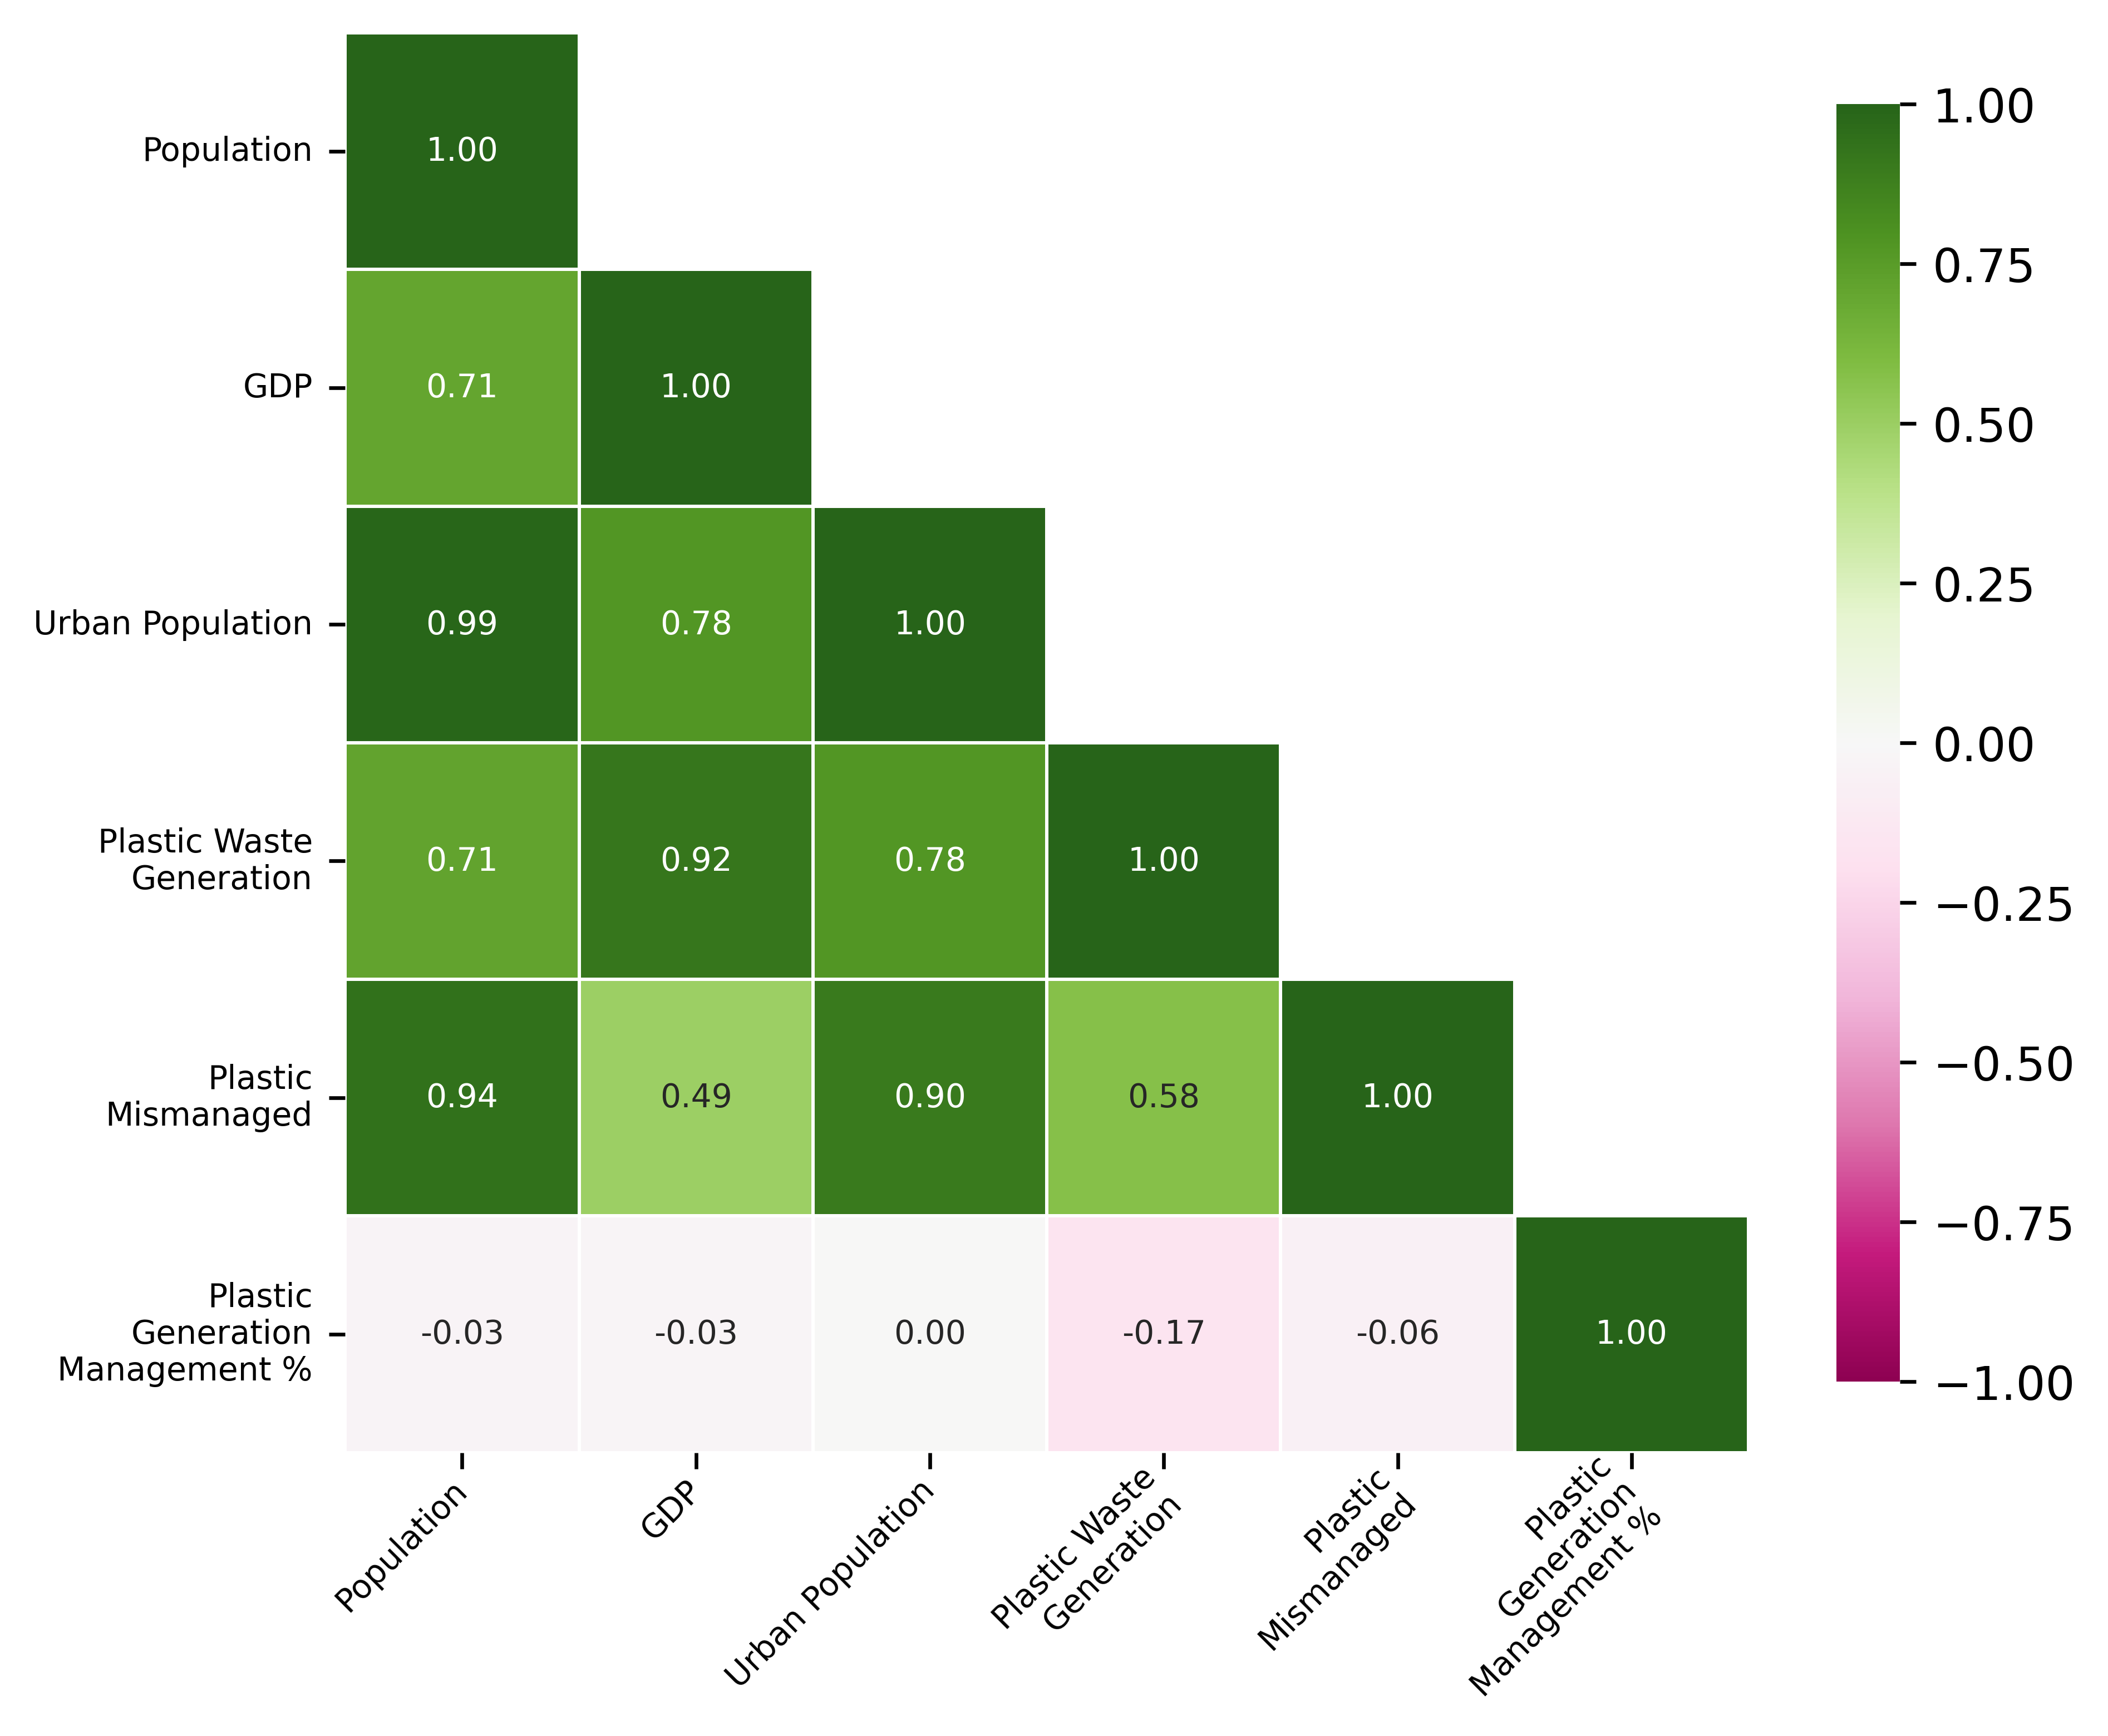
\includegraphics[width=0.8\linewidth]{figures/correlation_matrix.png}
	\caption{
		\centering
		Correlation matrix for the pooled \texttt{PWDriverFeatureSet} dataset. It summarizes pairwise association patterns across the pooled driver set.
	}
	\label{fig:correlation_matrix}
\end{figure}


Figure~\ref{fig:correlation_matrix} shows that GDP is strongly associated with plastic waste generation (\(r = 0.92\)). The correlation between urban population and plastic waste generation (\(r = 0.78\)) is stronger than that of total population (\(r = 0.71\)). Population and mismanaged plastic waste are also highly correlated (\(r = 0.94\)). In contrast, the percentage of plastic waste that is properly managed is nearly orthogonal to the scale variables and exhibits a weak negative correlation with plastic waste generation (\(r = -0.17\)).

Figure~\ref{fig:feature_importances} indicates that \textit{year} has the highest importance score (0.3348), followed by GDP (0.2984), suggesting that temporal trends and economic activity are the strongest predictors in this model. The importance of urban population (0.0868) is greater than rural population (0.0733) and total population (0.0450). This finding is consistent with recent work, which shows that urban areas contribute more to plastic waste generation due to higher consumption of single-use plastics and packaged goods~\cite{sen2026unveiling}.

\begin{figure}[H]
	\centering
	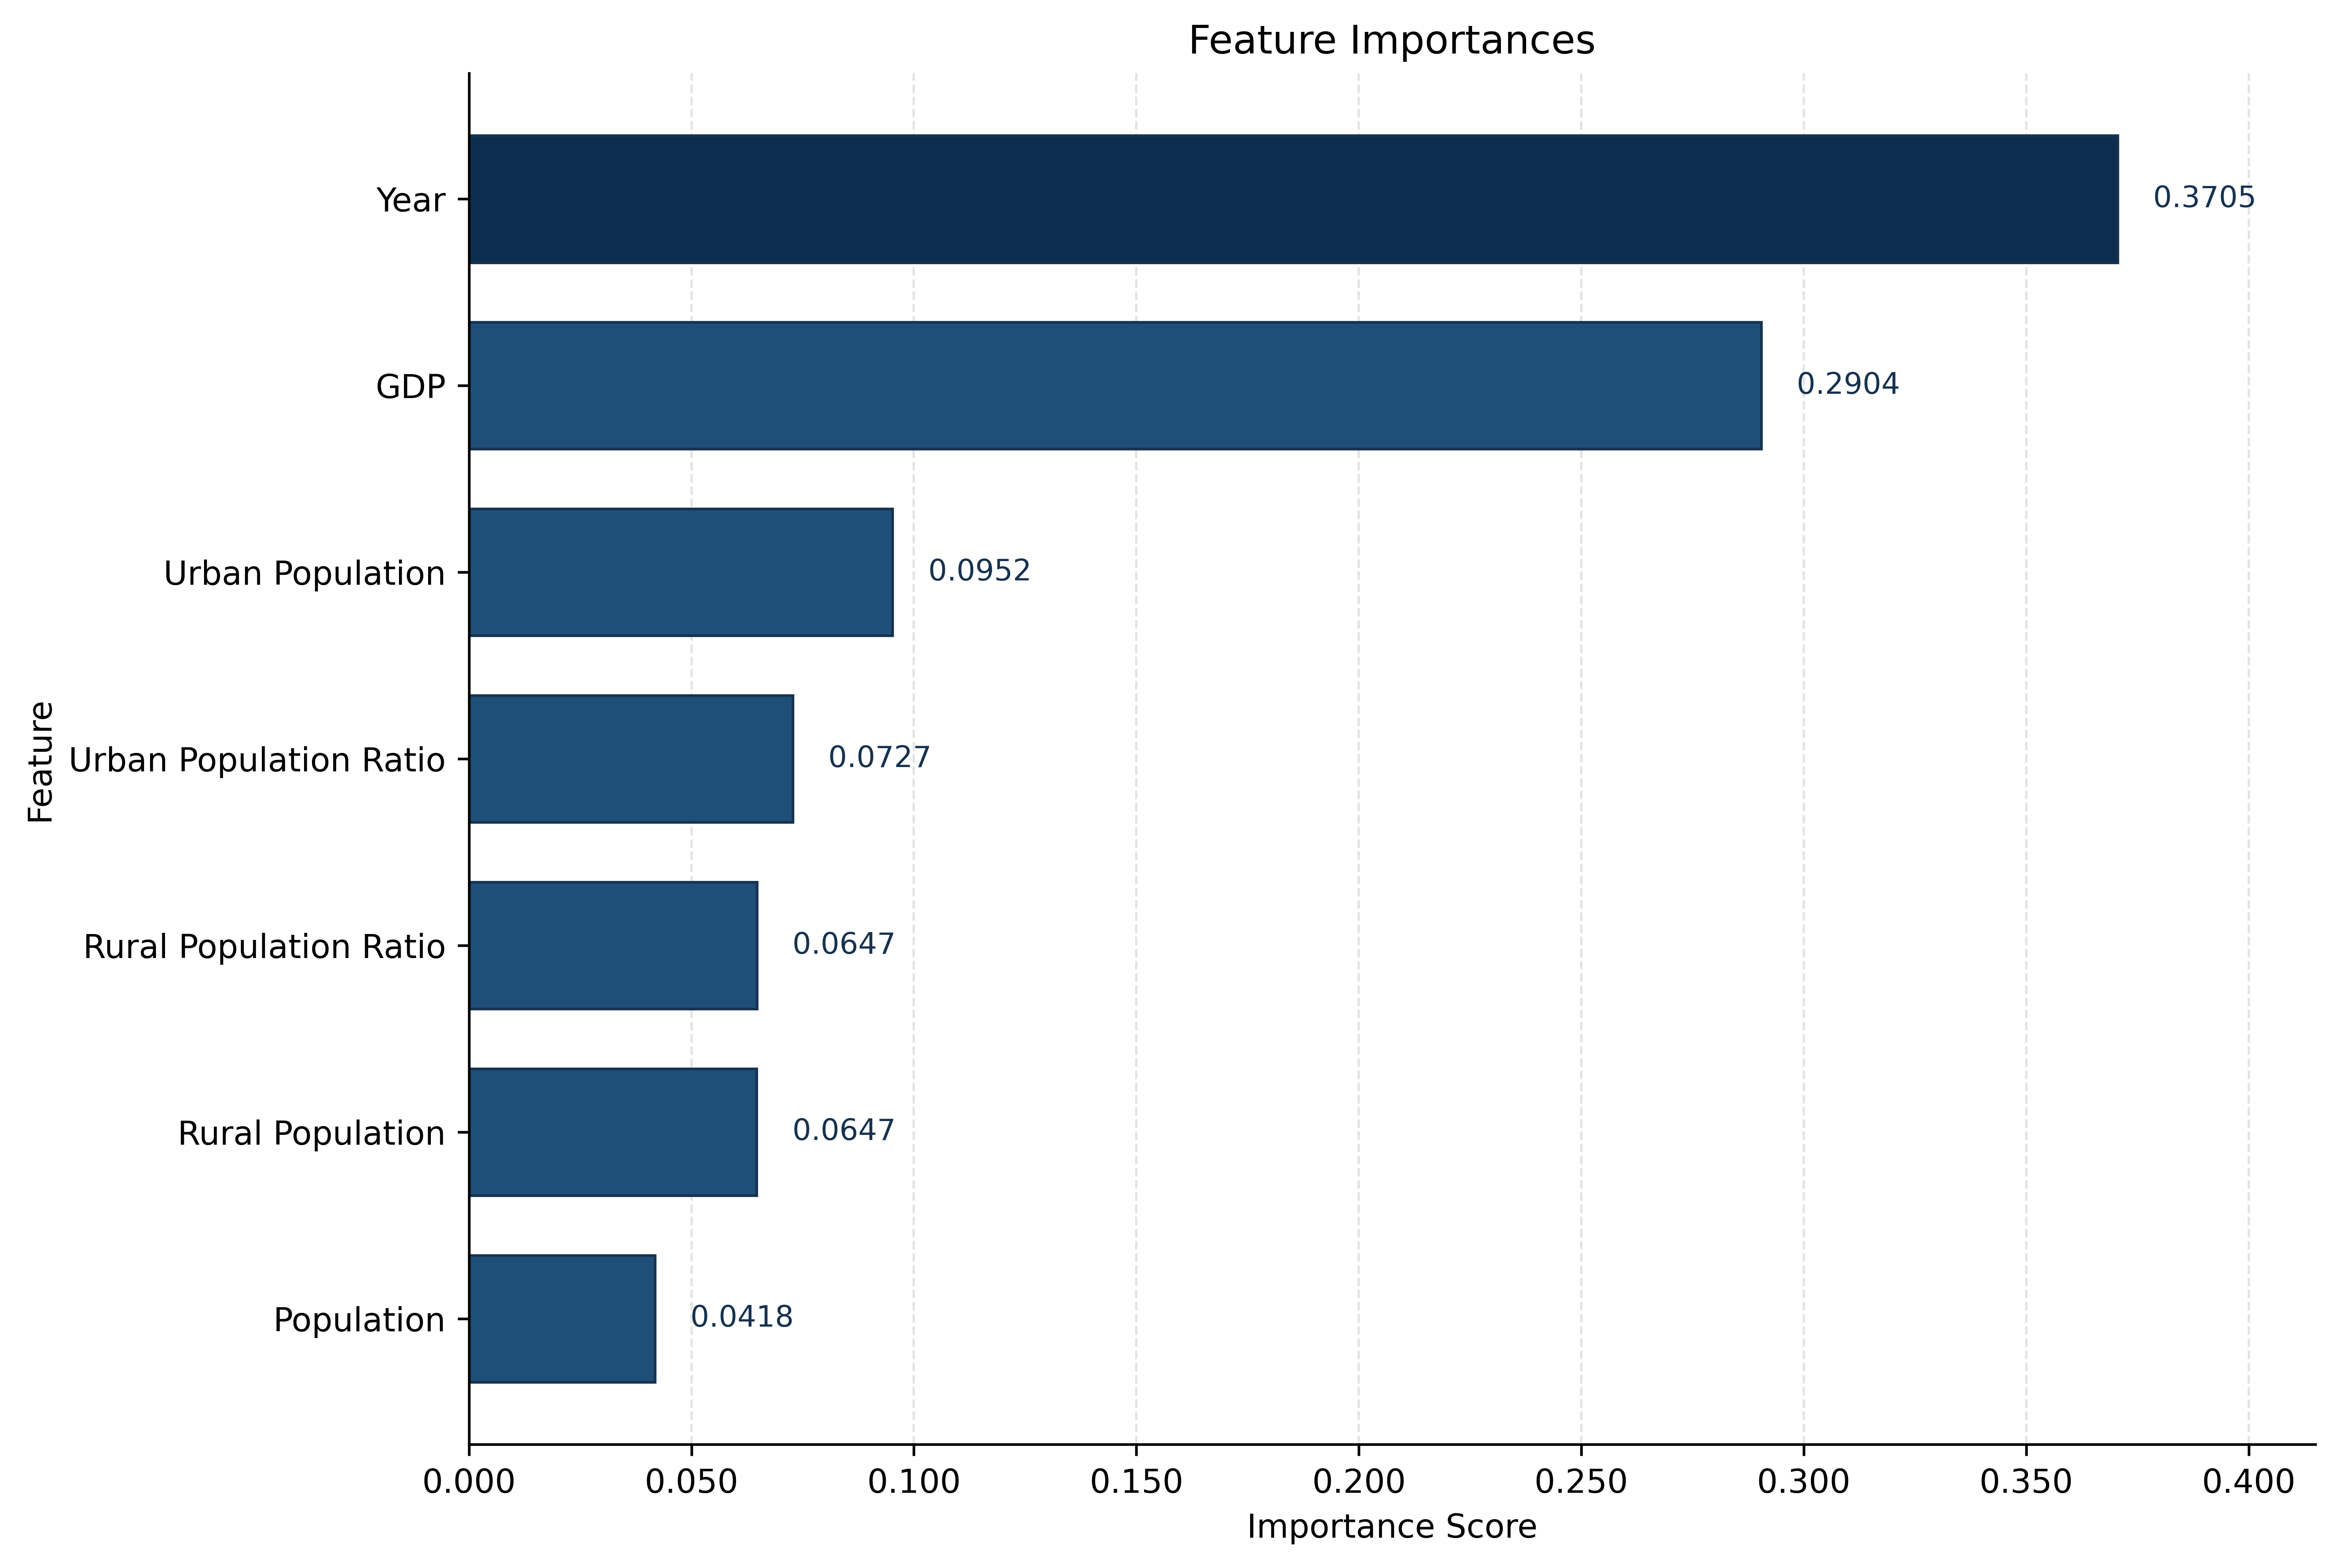
\includegraphics[width=1.0\linewidth]{figures/feature_importances.png}
	\caption{
		\centering
		Feature importances for the \texttt{PWGPredictors} dataset. This histogram shows the relative importance of each feature in predicting plastic waste generation.
	}
	\label{fig:feature_importances}
\end{figure}

